\documentclass[10pt, letterpaper]{report}
% !TeX program = xelatex
%==================PREAMBOLO=======================%
\usepackage[utf8]{inputenc}
\usepackage{psvectorian}
\usepackage{pgfplots}
\usepackage[Rejne]{fncychap}
\usepackage[export]{adjustbox}
\usepackage[T1]{fontenc}
\usepackage{lmodern}
\usepackage[shortlabels]{enumitem}
\usepackage{moresize}
\usepackage{graphicx} % Required for inserting images
\usepackage{hyperref}
\usepackage{listings}
\usepackage[table,xcdraw]{xcolor}
\usepackage{amssymb}
\usepackage{amsmath}
\usepackage[italian]{babel}
\usepackage{nicefrac, xfrac}
\usepackage{tikz}
\usepackage{mathrsfs} 
\usepackage{titletoc}
\usepackage{fancyhdr}
\usepackage{psvectorian,lipsum}
\usepackage{fourier-orns}
\usepackage{lipsum}
\usepackage[paper=a4paper,left=25mm,right=25mm,bottom=25mm,top=25mm]{geometry}
\definecolor{light-gray}{gray}{0.95}
\definecolor{cop}{HTML}{f7ecd7}
\definecolor{copAut}{HTML}{ababab}
\definecolor{copAut2}{HTML}{c3c3e6}
\definecolor{purcop}{HTML}{d0d3db}
\definecolor{sapienza}{HTML}{660f1d}
\definecolor{lightSapienza}{HTML}{e3d3d5}
\definecolor{darkgreen}{HTML}{008000}
\definecolor{cartaRiciclata}{HTML}{fcfcf7}
\newcommand{\redText}[1]{\color{red}#1\color{black}}
\newcommand{\code}[1]{\colorbox{light-gray}{\texttt{#1}}}
\newcommand{\codee}[1]{\colorbox{white}{\texttt{#1}}}
\newcommand{\K}{{\mathbb K}}
\newcommand{\notimplies}{%
  \mathrel{{\ooalign{\hidewidth$\not\phantom{=}$\hidewidth\cr$\implies$}}}}
\newcommand{\flowerLine}{ \begin{center}\decofourleft\hphantom{ }\decoone\hphantom{ }\decofourright\hphantom{}\hphantom{aa}
\decofourleft\hphantom{ }\decoone\hphantom{ }\decofourright\hphantom{}\hphantom{aa}
\decofourleft\hphantom{ }\decoone\hphantom{ }\decofourright\hphantom{}\hphantom{aa}
\decofourleft\hphantom{ }\decoone\hphantom{ }\decofourright\hphantom{}\hphantom{aa} 
\decofourleft\hphantom{ }\decoone\hphantom{ }\decofourright\hphantom{}\hphantom{aa}
\decofourleft\hphantom{ }\decoone\hphantom{ }\decofourright\hphantom{}\hphantom{aa}
\decofourleft\hphantom{ }\decoone\hphantom{ }\decofourright\hphantom{}\hphantom{aa}
\decofourleft\hphantom{ }\decoone\hphantom{ }\decofourright\hphantom{}\hphantom{aa}
\decofourleft\hphantom{ }\decoone\hphantom{ }\decofourright\hphantom{}\hphantom{aa}
\end{center}}
\definecolor{g}{RGB}{60, 50, 50}
\newcommand{\textg}[1]{\color{g}{\textbf{#1}}\color{black}}
\newcommand{\teo}[1]{{\large\color{sapienza}\textbf{Teorema #1 :\hphantom{a}}}}
\newcommand{\defi}[1]{{\large\color{sapienza}\textbf{Definizione #1 :\hphantom{a}}}}
\newcommand{\claim}[1]{{\color{sapienza}\textbf{Claim #1 :\hphantom{a}}}}
\newcommand{\lemma}[1]{{\color{sapienza}\textbf{Lemma #1 :\hphantom{a}}}}
\newcommand{\dimo}[1]{{\color{sapienza}\textbf{Dimostrazione #1 :\hphantom{a}}}}
\newcommand{\prop}[1]{{\color{sapienza}\textbf{Proposizione #1 :\hphantom{a}}}}
\newcommand\greybox[1]{%
  \vskip\baselineskip%
  \par\noindent\colorbox{light-gray}{%
    \begin{minipage}{\textwidth}#1\end{minipage}%
  }%
  \vskip\baselineskip%
}
\newcommand\sapbox[1]{%
  \vskip\baselineskip%
  \par\noindent\colorbox{lightSapienza}{%
    \begin{minipage}{\textwidth}#1\end{minipage}%
  }%
  \vskip\baselineskip%
}

\newcommand{\Z}{{\mathbb Z}}
\newcommand{\blank}{{\sqcup}}
\newcommand{\R}{{\mathbb R}}
\newcommand{\N}{{\mathbb N}}
\newcommand{\C}{{\mathbb C}}
\newcommand{\Sn}{{\mathcal S_n}}
\newcommand{\An}{{\mathcal A_n}}
\newcommand{\E}{{\mathcal E}}
\newcommand{\B}{{\mathcal B}}
\newcommand{\mcm}{{\text{mcm}}}
\newcommand{\rg}{{\text{rg}}}
\newcommand{\ve}{{\bar v}}
\newcommand{\spaz}{{\text{\hphantom{aa}}}}
\newcommand{\MCD}{{\text{MCD}}}
\newcommand{\tc}{{\text{ tale che }}}
\newcommand{\supp}{{\text{Supp}}}
\newcommand{\acc}{\\\hphantom{}\\}
\newcommand{\aut}{{\text{Aut}}}
\newcommand{\Span}{{\text{Span}}}
\newcommand{\End}{{\text{End}}}
\newcommand{\cen}{{\text{Centro}}}
\newcommand{\norm}{{\unlhd}}
\newcommand{\ciclS}{{\left \langle }}
\newcommand{\ciclE}{{\right \rangle }}
\newcommand{\boxedMath}[1]{\begin{tabular}{|c|}\hline \texttt{#1} \\ \hline\end{tabular} :}
\newcommand{\shell}[1]{\colorbox{black}{\textcolor{white}{\texttt{#1}}}}
\newcommand{\eqImportante}[1]{\begin{center}\huge\lefthand\hphantom{a}
    \normalsize\texttt{#1}
    \hphantom{aaa}\huge\righthand\end{center}}

\fancyhf{}
\pagestyle{fancy}
\usepackage{pgf-pie}  
\usetikzlibrary{positioning}

\renewcommand{\headrule}{%
\vspace{-8pt}\hrulefill
\raisebox{-2.1pt}{\quad\decothreeleft\decotwo\decothreeright\quad}\hrulefill}

%sta roba serve per il codice C
\definecolor{mGreen}{rgb}{0,0.6,0}
\definecolor{mGray}{rgb}{0.5,0.5,0.5}
\definecolor{mPurple}{rgb}{0.58,0,0.82}
\definecolor{backgroundColour}{rgb}{0.95,0.95,0.92}

\lstdefinestyle{CStyle}{
    backgroundcolor=\color{backgroundColour},   
    commentstyle=\color{mGreen},
    keywordstyle=\color{magenta},
    numberstyle=\tiny\color{mGray},
    stringstyle=\color{mPurple},
    basicstyle=\footnotesize,
    breakatwhitespace=false,         
    breaklines=true,                 
    captionpos=b,                    
    keepspaces=true,                 
    numbers=left,                    
    numbersep=5pt,                  
    showspaces=false,                
    showstringspaces=false,
    showtabs=false,                  
    tabsize=2,
    language=C
}
\lstdefinestyle{CppStyle}{
    backgroundcolor=\color{backgroundColour},   
    commentstyle=\color{mGreen}\ttfamily,
    morecomment=[l][\color{magenta}]{\#}
    keywordstyle=\color{blue}\ttfamily,
    numberstyle=\tiny\color{mGray},
    stringstyle=\color{red}\ttfamily,
    basicstyle=\ttfamily,
    breakatwhitespace=false,         
    breaklines=true,                 
    captionpos=b,                    
    keepspaces=true,                 
    numbers=left,                    
    numbersep=5pt,                  
    showspaces=false,                
    showstringspaces=false,
    showtabs=false,                  
    tabsize=2,
    language=C
}
\lstset{language=C++,
                basicstyle=\ttfamily,
                keywordstyle=\color{blue}\ttfamily,
                stringstyle=\color{red}\ttfamily,
                commentstyle=\color{green}\ttfamily,
                morecomment=[l][\color{magenta}]{\#}
}
%fine roba che serve per il codice C
\usepackage{minted}
 %TOGLI COMMENTO SE USI XELATEX
%\usepackage{fontspec}
\title{Automi, Calcolabilità e Complessità} %========TITOLO========%
\author{Marco Casu}
\date{\vspace{-5ex}}
\begin{document}
\usetikzlibrary{automata, arrows.meta, positioning}
%==================COPERTINA=======================%
\begin{titlepage}
    
\begin{center}
    %TOGLI COMMENTO SE USI XELATEX
   %\setmainfont{Palace Script MT}
   \HUGE Marco Casu\acc
    %\setmainfont{Grand Casino}
     %TOGLI COMMENTO SE USI XELATEX
    %\setmainfont{h Halfroad}
    \Huge \decothreeleft\hphantom{ }{\selectfont Automi, Calcolabilità e Complessità}\hphantom{ }\decothreeright
     %TOGLI COMMENTO SE USI XELATEX
   % \setmainfont{Times New Roman}
\end{center}
\thispagestyle{empty}
\begin{figure}[h]
    \centering{
        %l'immagine deve avere una risoluzione 2048x2048
        
\includegraphics[width=1\textwidth ]{images/copertina2.jpeg}
    }
\end{figure}
\vfill 
\centering 
\includegraphics[width=0.4\textwidth ]{../../preamble/Stemma_sapienza.png} \acc
\centering \Large \color{sapienza}Facoltà di Ingegneria dell'Informazione,
Informatica e Statistica\\
Dipartimento di Informatica
\end{titlepage}

%===================FINE COPERTINA======================%
\newpage
\pagecolor{cartaRiciclata}%\setmainfont{Algerian}
\Large
Questo documento è distribuito sotto la licenza 
\color{blue}\href{https://www.gnu.org/licenses/fdl-1.3.txt}{GNU}\color{black},  
è un resoconto degli appunti (eventualmente integrati con libri di testo) tratti dalle lezioni del corso di Automi, Calcolabilità e Complessità
\hphantom{a}per la laurea 
triennale in Informatica. Se dovessi notare errori, ti prego di segnalarmeli.
\newpage %\setmainfont{Times New Roman}
\normalsize
\tableofcontents 
\newpage

%==================FOOTER e HEADER=======================%
\fancyhf{}
\fancyhead[L]{\nouppercase{\leftmark}}
\fancyhead[R]{Sezione \thesection}
\fancyfoot[C]{\thepage}
\fancyfoot[L]{Appunti di Automi, Calcolabilità e Complessità}
\fancyfoot[R]{ Marco Casu}
%\fancyfoot[R]{\setmainfont{Palace Script MT}\huge Marco Casu \setmainfont{Times New Roman}}
%==================FOOTER e HEADER=======================%

%Ricorda del comando \flowerLine per separare le sottosezioni. Le sezioni si separano nelle diverse pagine

%==================INIZIO======================%
\chapter{Automi}
\section{Linguaggi Regolari}
Un \textit{automa a 
stati finiti} è, seppure limitato nella memoria e nella gestione 
dell'input, il più 
semplice modello di computazione. Un automa può interagire con l'input 
esclusivamente "scorrendolo" in maniera sequenziale.\acc 
\textbf{Esempio} : Si vuole modellare una semplice porta con sensore, che 
si apre quando qualcuno si trova nelle vicinanze.
\begin{center}
    \includegraphics[width=0.6\textwidth ]{images/porta.eps}
\end{center}
Un automa che modella il problema è il seguente :\begin{center}
    
    
    \begin{tikzpicture} [node distance = 6cm, on grid, auto]
        \node (aperta)[state, left] {aperta};
        \node (chiusa)[state, right = of aperta] {chiusa};
        \path [-stealth, thick]
        (aperta) edge [loop left]  node {rileva persone}()
        (chiusa) edge [loop right]  node {nessuno}()
        (aperta) edge [bend left] node {nessuno}   (chiusa)
        (chiusa) edge [bend left] node {rileva persone}   (aperta);
    \end{tikzpicture}
\end{center} 
Un automa ha alcuni stati speciali, come quello iniziale, indicato 
con un apposita freccia, e degli stati detti \textit{di accettazione}, 
ossia stati in cui deve necessariamente terminare la computazione per 
essere definita valida, vengono rappresentati con un doppio cerchio.
\acc 
Il modello di calcolo degli automi è riconducibile al concetto di 
\textit{linguaggio regolare}, che verrà formalizzato in seguito, 
segue ora una definizione formale di automa.\acc 
\defi{(DFA)} : Un DFA (Deterministic Finite Automa) è una 
5-tupla, $(Q,\Sigma,\delta, q_0, F)$ di cui\begin{itemize}
    \item $Q$ è l'insieme degli stati possibili 
    \item $\Sigma$ è l'alfabeto che compone le stringhe in input 
    \item $\delta$ è una mappa $Q\times \Sigma \rightarrow Q$ detta 
    \textit{funzione di transizione}. 
    \item $q_0\in Q$ è lo stato iniziale. 
    \item $F\subseteq Q$ è l'insieme degli stati di accettazione.
\end{itemize}
\begin{figure}[h!]
    \centering
    \begin{tikzpicture} [node distance = 3cm, on grid, auto]

        \node (q0) [state, initial, accepting, initial text = {}] {$q_1$};
        \node (q1) [state, above right = of q0] {$q_2$};
        \node (q2) [state, below right = of q1] {$q_3$};
        
        \path [-stealth, thick]
            (q0) edge node {0,1}   (q1)
            (q1) edge node {1}   (q2)
            (q1) edge [loop above]  node {0}()
            (q2) edge node {1,0} (q0);
        \end{tikzpicture}
        \caption{semplice automa}
        \label{fig:automaSemplice}
\end{figure}
Nell'esempio in figura \ref{fig:automaSemplice}, si ha che\begin{itemize}
    \item $Q=\{q_1,q_2,q_3\}$
    \item $\Sigma = \{0,1\}$
    \item $F=\{q_1\}$
    \item $q_0=q_1$
    \item $\delta =\;\;\; $ \begin{tabular}{c|c|c}
        & 0     & 1     \\ \hline
  $q_1$ & $q_2$ & $q_2$ \\ \hline
  $q_2$ & $q_2$ & $q_3$ \\ \hline
  $q_3$ & $q_1$ & $q_1$
  \end{tabular}
\end{itemize}
Sia $D$ un DFA, chiamiamo \textbf{linguaggio dell'automa}, e denotiamo 
$L(D)$, l'insieme delle stringhe che date in input a $D$ fanno si che 
$D$ termini su uno stato di accettazione.
\begin{figure}[h!]
    \centering
    \begin{tikzpicture} [node distance = 3cm, on grid, auto]
        \node (q0)[state, left, initial] {$q_1$};
        \node (q1)[state, right = of q0, accepting] {$q_2$};
        \path [-stealth, thick]
        (q0) edge [loop above]  node {0}()
        (q1) edge [loop above]  node {1}()
        (q0) edge [bend left] node {1}   (q1)
        (q1) edge [bend left] node {0}   (q0);
        \end{tikzpicture}
        \caption{il linguaggio di tale automa 
        risulta essere composto dalle stringhe che 
        terminano con $1$}
        \label{fig:automaSemplice2}
\end{figure}
Per definire formalmente un linguaggio di un automa, è 
necessario introdurre la \textbf{funzione di transizione estesa}:
$$ \delta^*(q,\epsilon)=\delta(q,\epsilon)$$
$$\delta^*(q,ax)=\delta^*(\delta(q,a),x)$$
dove
$$ a\in \Sigma,\;\;x\in \Sigma^*,\;\;\epsilon = \text{ stringa vuota}$$
$\Sigma^*$ è l'insieme di tutte le stringhe formate dall'alfabeto 
$\Sigma$. Passiamo ora alla definizione di \textbf{configurazione}, essa 
rappresenta lo stato dell'automa ad un certo punto della 
computazione, essa è formata da una coppia 
$$ Q\times \Sigma^*$$
Rappresentante uno stato, ed una stringa di input rimanente da 
computare.\acc 
Un \textbf{passo della computazione} in un automa rappresenta 
una transizione da una configurazione ad un altra, è una 
relazione binaria $\vdash_D : Q\times \Sigma^*$ tale che 
$$ 
(p,ax)\vdash_D (q,x)\iff \delta(p,a)=q \;\;\text{ dove }\;\;
p,q\in Q,\;\;a\in\Sigma,\;\;x\in\Sigma^*$$
Si può estendere la definizione di passo di computazione, 
considerando la sua \textit{chiusura transitiva} 
$\vdash_D^*$. Essa si ottiene aggiungendo a $\vdash_D$ tutte 
le coppie in $ Q\times \Sigma^*$ che rendono 
la relazione chiusa rispetto la riflessività e rispetto 
la transitività.
$$ \begin{matrix}
    (q,aby)\vdash_D (p,by) \;\land\;  
    (p,by)\vdash_D (ry) \implies 
    (q,aby)\vdash_D^*(r,y)
\end{matrix}$$
Ad esempio, nell'automa in figura \ref{fig:automaSemplice2}, 
risulta chiaro che 
$$\begin{cases}
    (q_1,011)\vdash_D (q_1,11)\\
    (q_1,11) \vdash_D (q_2,1)\\
    (q_2,1) \vdash_D (q_2,\epsilon)
\end{cases} \implies
(q_1,011) \vdash_D^* (q_2,\epsilon)$$
Inoltre$$ \begin{matrix}
    \delta^*(q_1,011) = \\ 
    \delta^*(q_1,11)  = \\ 
    \delta^*(q_2,1) = \\ 
    \delta^*(q_2,\epsilon) = q_2
\end{matrix}$$
Se non specificato diversamente, con $\epsilon$ verrà indicata 
la stringa vuota. Utilizzando le precedenti definizioni, è possibile definire formalmente 
quali sono gli input accettati da un DFA.\acc 
\defi{} : Sia $D=(Q,\Sigma,\delta, q_0, F)$ un DFA, e sia $x\in \Sigma^*$ una stringa, essa 
è \textbf{accettata} da $D$ se $$ \delta^*(q_0,x)\in F$$
Il \textbf{linguaggio riconosciuto} da $D$ è \eqImportante{$ L(D)=\{x\in \Sigma^*|\delta^*(q_0,x)\in F\}$}
\defi{(Linguaggi Regolari)} : L'insieme dei linguaggi regolari, denotato $REG$, contiene tutti 
i linguaggi, tali che esiste un DFA che li ha come linguaggi riconosciuti.
\eqImportante{$ REG = \{L\;\;|\;\;\exists D=(Q,\Sigma,\delta, q_0, F) \text{ t.c. } L\in \Sigma^* \land L(D)=L\}$}
Uno fra gli scopi di questo corso riguarda il capire come progettare automi, e capire se, 
ogni linguaggio è regolare, o ce ne sono alcuni che non possono essere riconosciuti da 
alcun possibile DFA. 
\subsection{Esempi di DFA}
Vediamo in questa sezione alcuni semplici esempi di DFA.\acc 
\textbf{Esempio 1)} Si vuole progettare un DFA che accetti il seguente linguaggio 
$$ \{x\in\{0,1\}^* \;|\;w_h(x)\ge 3 \}$$
Si ricordi come 
$$ w_h(x) = \text{ occorrenze di 1 in }x$$
\begin{figure}[h!]
    \centering
    \begin{tikzpicture} [node distance = 2cm, on grid, auto]
        \node (q0)[state, left, initial] {$q_0$};
        \node (q1)[state, right = of q0] {$q_1$};
        \node (q2)[state, right = of q1] {$q_2$};
        \node (q3)[state, right = of q2, accepting] {$q_3$};
        \path [-stealth, thick]
        (q0) edge [loop above]  node {0}()
        (q1) edge [loop above]  node {0}()
        (q2) edge [loop above]  node {0}()
        (q3) edge [loop right]  node {1,0}()
        (q0) edge [bend left] node {1}   (q1)
        (q1) edge [bend left] node {1}   (q2)
        (q2) edge [bend left] node {1}   (q3);
        \end{tikzpicture}
        \caption{Esempio (1) di DFA}
        \label{fig:DFAExample1}
\end{figure}
Una volta progettato il DFA, è anche importante dimostrarne la correttezza, ossia dare una prova 
matematico che l'automa in questione accetti il linguaggio.\begin{itemize}
    \item Se $x\in L(D)$ allora $D$ accetta $x$
    \item Se $D$ accetta $x$ allora $w_h(x)\ge 3$
\end{itemize}
In questo, e nei seguenti casi, essendo i DFA estremamente semplici, risulta ovvio che 
accettino il dato linguaggio, in casi più avanzati, sarà necessario fornire una dimostrazione 
rigorosa.\acc 
\textbf{Esempio 2)} Si vuole progettare un DFA che accetti il seguente linguaggio 
$$ \{x\in\{0,1\}^* \;|\;x=1y \land y \in  \{0,1\}^*\}$$
Appunto sulla notazione : Se $a\in \Sigma^*$ e $b\in \Sigma^*$, allora con $ab$ si 
denota la concatenazione di stringhe.\acc
\begin{figure}[h!]
    \centering
    \begin{tikzpicture} [node distance = 2cm, on grid, auto]
        \node (q0)[state, left, initial] {$q_0$};
        \node (q1)[state, below = of q0] {$q_1$};
        \node (q2)[state, right = of q0, accepting] {$q_2$};
        \path [-stealth, thick]
        (q1) edge [loop left]  node {0,1}()
        (q2) edge [loop above]  node {0,1}()
        (q0) edge [bend left] node {0}   (q1)
        (q0) edge [bend left] node {1}   (q2);
        \end{tikzpicture}
        \caption{Esempio (2) di DFA}
        \label{fig:DFAExample2}
\end{figure}\acc 
Nell'esempio (2), quando dallo stato $q_0$ il DFA riceve in input $0$, la computazione cade su uno stato 
"buco nero", dalla quale non si può uscire a prescindere dall'input, l'operazione che fa 
cadere in questo stato è da considerarsi "non definita" in quanto non porterà mai la computazione 
a terminare su uno stato accettabile, è quindi comodo rimuovere tale stato dal diagramma.
\begin{figure}[h!]
    \centering
    \begin{tikzpicture} [node distance = 3cm, on grid, auto]
        \node (q0)[state, left, initial] {$q_0$};
        \node (q2)[state, right = of q0, accepting] {$q_2$};
        \path [-stealth, thick]
        (q2) edge [loop above]  node {0,1}()
        (q0) edge [bend left] node {1}   (q2);
        \end{tikzpicture}
        \caption{Esempio (2.1) di DFA}
        \label{fig:DFAExample2.1}
\end{figure}\acc 
Anche in questo caso la dimostrazione della correttezza risulta banale.\acc 
\textbf{Esempio 3)} Si vuole progettare un DFA che accetti il seguente linguaggio 
$$ \{x\in\{0,1\}^* \;|\;x=0^n1,\;\;n\in \N\}$$
Con $0^n1$ si intende una stringa che abbia un numero naturale di di $0$ (quindi, almeno uno), e 
che termini con $1$.
\begin{figure}[h!]
    \centering
    \begin{tikzpicture} [node distance = 3cm, on grid, auto]
        \node (q0)[state, left, initial] {$q_0$};
        \node (q1)[state, right = of q0] {$q_1$};
        \node (q2)[state, right = of q1, accepting] {$q_2$};
        \path [-stealth, thick]
        (q0) edge [loop below]  node {1}()
        (q1) edge [loop above]  node {0}()
        (q2) edge [loop right]  node {1}()
        (q0) edge  node {0}   (q1)
        (q1) edge  node {1}   (q2)
        (q2) edge [bend left] node {0}   (q1);
        \end{tikzpicture}
        \caption{Esempio (3) di DFA}
        \label{fig:DFAExampl3}
\end{figure}\acc 
\textbf{Dimostrazione di correttezza} : Sia $x$ una stringa data in input al DFA \begin{itemize}
    \item se $x$ ha un numero naturale di $0$, sicuramente ne ha almeno 1, quindi 
    ad un certo punto della computazione passerà dallo stato $q_0$ allo stato $q_1$
    \item la computazione, una volta passata per lo stato $q_1$, non tornerà più 
    nello stato $q_0$, quindi le configurazioni successive si troveranno solamente in uno stato 
    fra $q_1$ e $q_2$. 
    \item supponiamo $x$ termini con $1$ : \begin{itemize}
        \item Se la configurazione si trova su $q_1$, si ha $\delta(q_1,1)=q_2$, la computazione 
        termina su uno stato accettabile. 
        \item Se la configurazione si trova su $q_2$, si ha $\delta(q_2,1)=q_2$, la computazione 
        termina su uno stato accettabile. 
    \end{itemize}
    In entrambi i casi, essendo che l'automa termina su uno stato accettabile, esso riconosce 
    il linguaggio, che risulta quindi, regolare. $\blacksquare$
\end{itemize}
\flowerLine 
\section{Operazioni sui Linguaggi}
Lo studio delle proprietà dei linguaggi regolari può fornire opportune accortezze
utili nella progettazione di automi, siccome i linguaggi sono insiemi di stringhe costruiti 
su un alfabeto $\Sigma$, essi godono delle operazioni insiemistiche.\acc
Risulta utile definire formalmente la concatenazione fra stringhe, siano 
$$ x = a_1,a_2\dots,a_n\;\;\;\;\;\;\;\;\;\;\;\;y = b_1,b_2\dots,b_n $$
due stringhe, esse possono essere concatenate 
$$xy=  a_1,a_2\dots,a_n,b_1,b_2\dots,b_n $$
L'operazione di concatenazione non è commutativa, può essere definita ricorsivamente in tal 
modo : 
$$ x(ya) = (xy)a$$ 
dove 
$$x,y\in \Sigma^*\;\;\;\;\;\;\;\;\;a\in \Sigma$$
Siano $L_1,L_2$ due 
linguaggi regolari in $REG$ (per semplicità, definiti su uno stesso alfabeto $\Sigma$), e 
sia $n$ un numero naturale, sono 
definite su di essi le seguenti operazioni : \begin{itemize}
    \item \textbf{unione} : $L_1\cup L_2 = \{x\in\Sigma^*\;|\;x\in L_1\lor x\in L_2\}$
    \item \textbf{intersezione} : $L_1\cap L_2 = \{x\in\Sigma^*\;|\;x\in L_1\land x\in L_2\}$
    \item \textbf{complemento} : $\lnot L_1=\{x\in\Sigma^*\;|\;x\notin L_1\}$
    \item \textbf{concatenazione} : $L_1 \circ L_2 = \{xy\;|\;x\in L_1\land y\in L_2\}$
    \item \textbf{potenza} : $L_1^n = \smash{\underbrace{L_1\circ L_1\circ L_1,\dots\circ L_1}_{n\ \text{volte}}}\vphantom{1}$\acc
    \item \textbf{star} : $L_1^* = \{x_1,x_2\dots,x_k\;|\; k\in \Z^+ \land x_i \in L_1\}$ \\ 
    Si può definire anche diversamente $$L_1^* = \bigcup_{k=0}^\infty L_1^k $$
\end{itemize}
Una particolarità dei linguaggi regolari $REG$, è che sono chiusi rispetto a tutte le operazioni appena elencate.
$$\begin{matrix}
    L_1\cup L_2 \in REG && L_1\circ L_2 \in REG &&
    L_1\cap L_2 \in REG \\ \\ L_1^n \in REG &&
    \lnot L_1 \in REG && L_1^* \in REG
\end{matrix}$$
\textit{Esempio di concatenazione e potenza} : 
$$\Sigma= \{a,b\}\;\;\;\; L_1 = \{a,ab,ba\}\;\;\;\; L_2 = \{ab,b\}\;\;\;\; L = \{a,ab,ba\}$$
$$L_1\circ L_2 = \{aab,ab,abab,abb,baab,bab\} $$
$$ L^2=\{aa,aab,aba,abab,abba,baa,baba\}$$
\end{document}